
\subsection{fstat}


\textbf{fstat}主要功能在文件系统章节已经介绍,用于由文件描述符,获取文件当前状态。
所以本小节将从fstat所用到的\textbf{stat结构体},与\textbf{利用fd查找文件}两个角度出发,来解释fstat函数在操作系统文件部分中的实现和应用。\\

\subsubsection{系统调用原型}
\begin{lstlisting}[language={Rust}, 
	caption={os/src/syscall/fs.rs}]
    pub fn sys_fstat(fd: usize, statbuf: *mut u8);
\end{lstlisting}
参数解释:\\
fd:文件描述符(file descriptor),是一个非负整数,用于唯一标识打开的文件。\\
statbuf:一个指向stat结构的指针,用于接收文件详细信息(指向内容如代码片段9.20)。\\
返回值: 执行成功则返回SUCCESS,失败返回errno并跳入。成功和失败的判定是在于有没有通过fd找到文件,且返回相关的stat信息。\\

\subsubsection{fstat流程}
根据fstat系统调用的功能,我们可以写出fstat函数的流程与伪代码。需要注意的是,传入的fd可能本身不存在,所以为了提升鲁棒性,我们还需要判断fd是否为正,否则直接跳入errno。
例外:fd为AT_FDCWD(-100),表明当filename为相对路径的情况下,将当前进程的工作目录设置为起始路径。此时我们则需要对当前inode进行克隆,防止死锁。
\begin{figure}[H]
    \centering
    \scalebox{0.18}{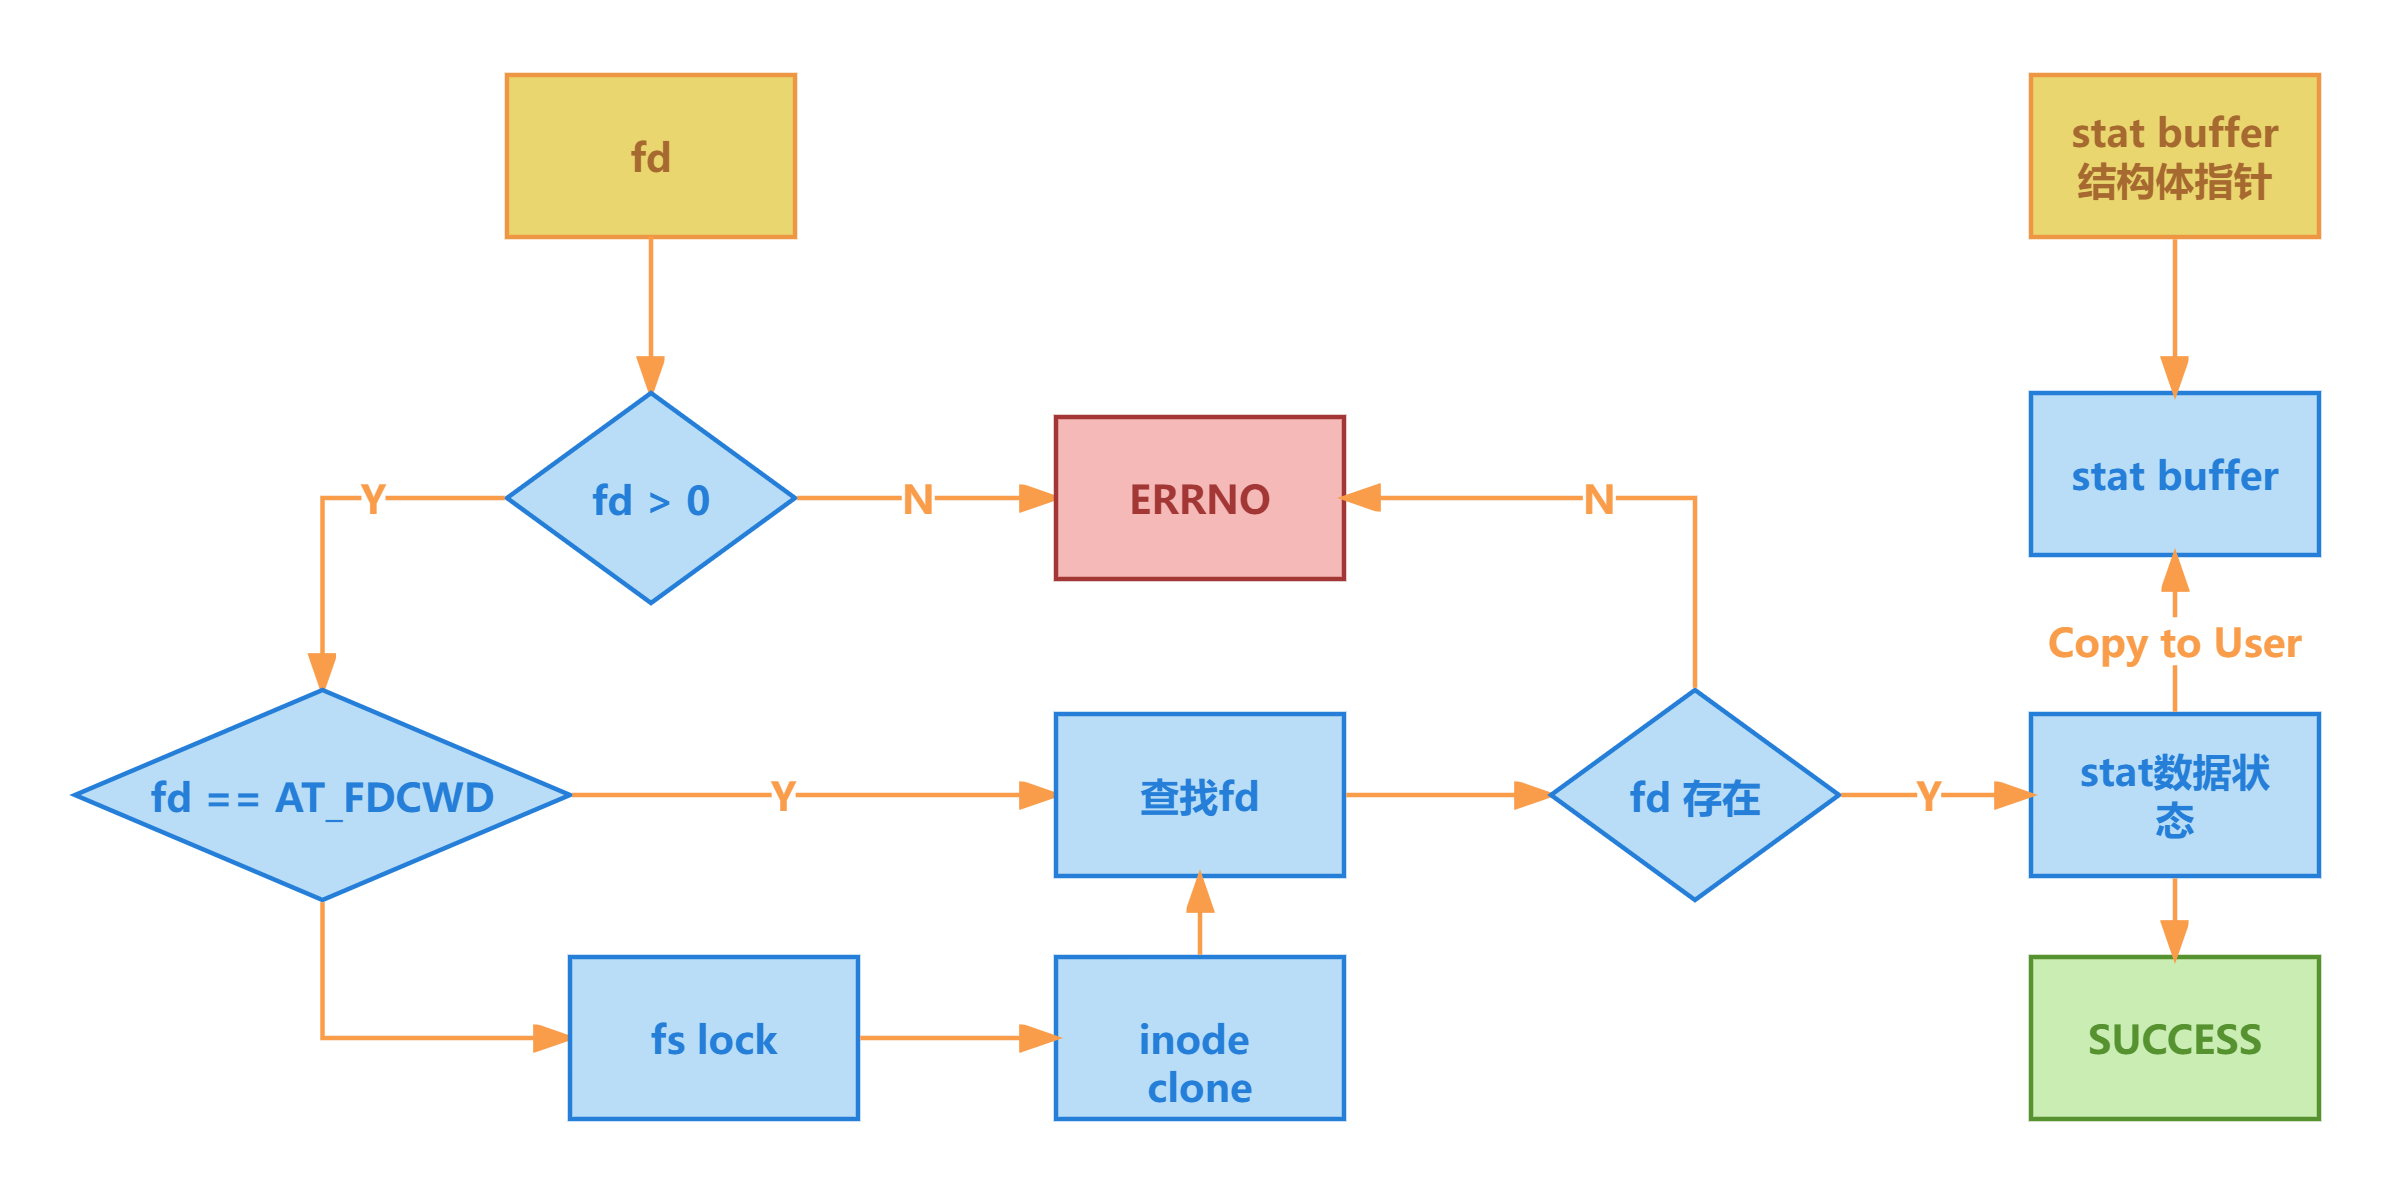
\includegraphics{figures/09-04-fstat-流程图.png}}
    \caption{fstat流程框图,黄色框代表输入,红色与绿色框分别是两种不同的输出,蓝色框为流程}
\end{figure}

\begin{algorithm}[tb]
    \caption{fstat}
    \label{alg:algorithm}
    \textbf{Input}: fd, statbuf\\
    \textbf{Output}: SUCCESS~or~ERRNO
    \begin{algorithmic}[1] %[1] enables line numbers

        \State Let $task=current~task$.
        \State Let $token=user~token$.
        \If{$fd<0$~or~$fd~unmatched$}
        \State \textbf{return} $ERRNO$
        \Else \If{$fd$~\textbf{equal}~$AT\underline{~~}FDCWD$}
        \State lock and clone, copy stat to buf
        \Else
        \State copy stat to buf
        \EndIf
        \State \textbf{return} $SUCCESS$
        \EndIf
    \end{algorithmic}
\end{algorithm}


这里我们也给出stat的结构体供大家参考。

\begin{lstlisting}[language={Rust}, 
	caption={stat示意结构体}]
    struct stat {
    dev_t     st_dev;         // 文件所在设备的设备号
    ino_t     st_ino;         // 文件的i节点号
    mode_t    st_mode;        // 文件的访问权限
    nlink_t   st_nlink;       // 文件的硬链接数
    uid_t     st_uid;         // 文件所有者的用户ID
    gid_t     st_gid;         // 文件所有者的组ID
    dev_t     st_rdev;        // 如果文件是特殊字符设备或块设备,保存设备号
    off_t     st_size;        // 文件的大小(常以字节为单位)
    blksize_t st_blksize;     // 文件I/O缓冲区大小
    blkcnt_t  st_blocks;      // 分配给文件的块数
    time_t    st_atime;       // 文件的最近访问时间
    time_t    st_mtime;       // 文件的最近修改时间
    time_t    st_ctime;       // 文件的最近更改时间(包括权限和归属人等)
};
\end{lstlisting}


\subsubsection{fstat代码详解}

第一步,获取当前线程,老生常谈,不多介绍。
\begin{lstlisting}[language={Rust}, 
	caption={获取线程}]
    let task = current_task().unwrap();
    let token = task.get_user_token();
\end{lstlisting}
第二步,搜索fd是否存在。本处省略了对fd大于0的判断。
1.首先,通过match语句对文件描述符进行匹配。
2.如果匹配到的文件描述符是AT_FDCWD,代表当前工作目录的文件描述符,那么将通过task.fs.lock().working_inode.as_ref().clone()获取到当前任务(task)的文件系统(fs)的锁,然后获取到工作inode(working inode)的引用,并进行克隆(clone)得到一个新的file_descriptor。
3.如果匹配到的文件描述符不是AT_FDCWD,则会执行下面的代码块。
4.在下面的代码块中,首先获取到当前任务的文件表(fd_table)的锁,并使用get_ref(fd)方法获取到指定文件描述符的引用。
5.如果获取成功(Ok),则克隆(clone)该文件描述符,并将克隆得到的新的file_descriptor赋值给file_descriptor变量。
如果获取失败(Err),则会返回一个表示错误码(errno)的值。
\begin{lstlisting}[language={Rust}, 
	caption={fd查找}]
    let file_descriptor = match fd {
        AT_FDCWD => task.fs.lock().working_inode.as_ref().clone(),
        fd => {
            let fd_table = task.files.lock();
            match fd_table.get_ref(fd) {
                Ok(file_descriptor) => file_descriptor.clone(),
                Err(errno) => return errno,
            }
        }
    };
\end{lstlisting}
第三步,将fd搜索到的stat信息,写入用户定义的buffer中。我们直接使用copy_to_user函数即可。函数结束,顺利返回SUCCESS。
\begin{lstlisting}[language={Rust}, 
	caption={赋值stat~buffer}]
    copy_to_user(token, &file_descriptor.get_stat(), statbuf as *mut Stat);
    return SUCCESS;
\end{lstlisting}
